\documentclass[conference]{IEEEtran}
\usepackage{amsmath,amssymb}
\usepackage{graphicx}
\usepackage{booktabs}
\usepackage{multirow}
\usepackage{siunitx}
\usepackage{url}
\usepackage[hidelinks]{hyperref}
\usepackage{cite}

\begin{document}

\title{Vision-Only Landing of a Quadcopter on a Moving Ground Vehicle:\\
Attitude-Compensated Estimation and a Closed-Loop Simulation Study in ROS~2}

\author{\IEEEauthorblockN{Dimuthu Wickramanayake}
\IEEEauthorblockA{Email: \href{mailto:dimuthu.billa@gmail.com}{dimuthu.billa@gmail.com}}}

\maketitle

\begin{abstract}
We study the landing of a quadcopter on a moving ground vehicle using only a downward-facing
monocular camera and a landing pad carrying three ArUco markers of different sizes, with no
communication link between the aircraft and the vehicle. The system is implemented as a set of
ROS~2 nodes: a marker detector that fuses all visible markers into one pad pose, a relative-state
estimator, and a landing state machine that ends with a motor cut and a short free fall onto the
pad. Because a multirotor must tilt to accelerate, the pose measured in the camera frame is
rotated by the aircraft attitude into a gravity-aligned frame before it is used, and the pad's
position and velocity are tracked with a constant-velocity Kalman filter. We evaluate three
estimator variants on identical rendered camera images in a closed-loop simulator with wind,
camera latency and flight-controller state errors. In a hover test with the pad passing at
1--\SI{9}{m/s}, the filtered estimator's speed RMSE is 0.07--\SI{0.14}{m/s}, against
0.48--\SI{0.98}{m/s} for unfiltered variants. Over 22\,092 in-flight detections, the median
position error of the camera-frame estimate grows from \SI{2.6}{cm} below \ang{2} of tilt to
\SI{1.62}{m} at \ang{20}--\ang{30}, while the attitude-compensated estimates stay between 1.0
and \SI{3.2}{cm}. In 28 closed-loop trials per variant across seven vehicle motions, the
camera-frame variant never landed, the attitude-compensated variant landed 6 times and the
filtered variant 7 times, at a mean distance of \SI{6.3}{cm} from the pad centre. No landing
succeeded for weaving, stop-and-go or \SI{4.5}{m/s} vehicle motion. The code, simulator and
data are open source.
\end{abstract}

\begin{IEEEkeywords}
quadcopter, autonomous landing, moving platform, fiducial markers, ArUco, Kalman filter, ROS~2
\end{IEEEkeywords}

%% ------------------------------------------------------------------------------------------
\section{Introduction}

Multirotor aircraft can take off and land vertically and hover in place, which makes them
useful for inspection, delivery and search tasks. Their short flight time makes it attractive to
launch and recover them from a ground vehicle, but landing on a vehicle that is moving is
considerably harder than landing on the ground. The aircraft must find the landing pad,
estimate where it is and how fast it is moving, match that motion despite wind, and touch down
on a small area.

Many systems solve part of this problem by sharing state between the aircraft and the vehicle,
for example by sending the vehicle's GNSS position or odometry over a radio link. Such a link
cannot always be relied on. This paper therefore considers the case in which the aircraft
carries everything it needs: one downward-facing camera, the attitude and velocity estimate of
its own flight controller, and a known pattern of fiducial markers on the vehicle.

The work builds on an earlier prototype by the author and colleagues~\cite{wickramanayake2019landing},
which used a Raspberry Pi for vision, an Arduino Nano for flight control and a landing pad
with three ArUco markers of different sizes, and which measured the speed of a moving target
from a hovering aircraft. Closing the loop---flying the aircraft from the vision estimate all
the way to touchdown---was left as future work. This paper addresses that step.

The specific contributions are:
\begin{enumerate}
\item A complete vision-only landing pipeline in ROS~2 (Jazzy): multi-marker pad detection,
attitude-compensated relative-state estimation with a constant-velocity Kalman filter, and a
landing state machine with a predicted-impact check before the motor cut.
\item A closed-loop simulator that renders the downward camera image so that the actual
OpenCV ArUco detector runs in the loop, together with quadrotor and vehicle dynamics, gusting
wind, camera latency and flight-controller state errors. It runs without Gazebo or a GPU.
\item A controlled comparison of three estimator variants on identical images, quantifying how
estimation error depends on aircraft tilt and how each variant performs in closed-loop landing
across seven vehicle motions.
\item A measurement of how the three-marker pad's detection rate varies with height.
\end{enumerate}

All software, the simulator, the experiment scripts and the raw results are available at
\url{https://github.com/deBilla/moving-target-landing-ros2}.

%% ------------------------------------------------------------------------------------------
\section{Related Work}
\label{sec:related}

Surveys of autonomous UAV landing are given by Gautam \emph{et al.}~\cite{gautam2014survey},
who compare GPS-based and vision-based methods and the control approaches used with them, by
Kong \emph{et al.}~\cite{kong2014vision}, who classify vision-based landing systems, and more
recently by Xin \emph{et al.}~\cite{xin2022vision}, who separate static, dynamic (vehicle- and
ship-based) and complex landing scenarios. We organise the work most relevant here into five
groups.

\subsection{Vision-guided landing on moving targets}
Saripalli \emph{et al.}~\cite{saripalli2003visually} demonstrated real-time vision-guided
landing of an autonomous helicopter on a static target, and Saripalli and
Sukhatme~\cite{saripalli2006landing} extended it to a moving target, recognising the target
with Hu's moment invariants and tracking it with a Kalman filter. Wenzel
\emph{et al.}~\cite{wenzel2011automatic} showed a miniature UAV taking off from, tracking and
landing on a moving carrier vehicle. Heriss\'e \emph{et al.}~\cite{herisse2012landing} used
optical flow together with an IMU in a nonlinear controller that stabilises a VTOL aircraft
relative to a moving textured platform, with a stability proof and quadrotor experiments. Lee
\emph{et al.}~\cite{lee2012autonomous} applied image-based visual
servoing~\cite{chaumette2006visual}, producing velocity references from image-space errors for
an adaptive sliding-mode controller. Lee, Jung and Shim~\cite{lee2016vision} detected a
coloured marker on a vehicle on board in real time and landed on the moving vehicle in outdoor
flights. Falanga \emph{et al.}~\cite{falanga2017vision} landed a quadrotor on a moving platform
using only onboard sensing and computation, combining platform detection, motion estimation
and trajectory planning on low-cost hardware. Ghommam and Saad~\cite{ghommam2017autonomous}
used a single downward camera for relative position and divided the landing into search,
homing and landing phases with adaptive backstepping control. Gautam
\emph{et al.}~\cite{gautam2022autonomous} used pure-pursuit guidance with a closing-velocity
controller and landed on a slowly moving target in 22 of 27 field trials.

\subsection{Relative-state estimation}
Many of these systems estimate the platform's relative position and velocity with a
filter~\cite{kalman1960new}. Borowczyk \emph{et al.}~\cite{borowczyk2017autonomous} used a
Kalman filter on relative position and velocity and landed a commercial quadcopter repeatedly
on the roof of a car travelling at high speed. Araar \emph{et al.}~\cite{araar2017vision}
designed a landing pad together with a relative pose estimator for it, and fused the visual
pose with inertial measurements to obtain a high-rate estimate. Paris
\emph{et al.}~\cite{paris2020dynamic} used an extended Kalman filter that switches from
(simulated) GNSS at long range to fiducial markers at short range. Feng
\emph{et al.}~\cite{feng2018autonomous} localised a mobile platform with a Kalman filter and a
gimbaled camera. A gimbal, or fusion with inertial data, is one way to account for the fact that a body-fixed
camera rotates with the aircraft. In this paper we quantify the size of that effect on a fixed
downward camera during pursuit, and its consequence for closed-loop landing.

\subsection{Trajectory planning and control}
Several works plan the approach explicitly. Vlantis \emph{et al.}~\cite{vlantis2015quadrotor}
used nonlinear model predictive control (MPC) with a forward-looking camera to land on an
inclined platform carried by a mobile robot, keeping the platform in the field of view as a
constraint. Feng \emph{et al.}~\cite{feng2018autonomous} and Guo
\emph{et al.}~\cite{guo2022autonomous} used MPC guidance, the latter re-planning with a
variable sampling time as the aircraft nears the platform. Hu and Mishra~\cite{hu2019time}
generated time-optimal landing trajectories onto a heaving and pitching platform. Paris
\emph{et al.}~\cite{paris2020dynamic,paris2021autonomous} addressed fast landing in turbulent
wind, first with receding-horizon planning and robust control and then with explicit wind
estimation. The landing task of the Mohamed Bin Zayed International Robotics Challenge (MBZIRC)
2017 produced field-tested systems: Baca \emph{et al.}~\cite{baca2019autonomous} predicted the
vehicle's motion with a nonlinear model and used MPC to land on a car at \SI{15}{km/h}, and Beul
\emph{et al.}~\cite{beul2019team} combined camera-based perception with fast trajectory
planning for the same task. Daly \emph{et al.}~\cite{daly2015coordinated} took a different
approach in which the aircraft and a ground vehicle cooperate through a decentralised
controller, which requires communication between them.

\subsection{Learning-based landing}
Polvara \emph{et al.}~\cite{polvara2018toward} trained a hierarchy of deep Q-networks to land on
a static marker from low-resolution downward images. Rodriguez-Ramos
\emph{et al.}~\cite{rodriguezramos2019deep} trained a DDPG agent in a Gazebo-based
framework~\cite{koenig2004design} for landing on a moving platform and transferred it to real
flights. Ladosz \emph{et al.}~\cite{ladosz2024autonomous} learned landing on a moving platform
end-to-end from camera images, including vertical velocity control, and reported better
performance in simulation than with hand-extracted relative position and velocity features.

\subsection{Fiducial markers and landing pads}
Square fiducial markers such as AprilTag~\cite{olson2011apriltag,wang2016apriltag} and
ArUco~\cite{garrido2014aruco,romero2018speeded} give a full 6-DOF pose from a single image and
are widely used for landing pads. Planar pose can be computed accurately with infinitesimal
plane-based pose estimation (IPPE)~\cite{collins2014infinitesimal}. A known problem for landing
is that a single marker is either too small to detect from high up or too large to stay in the
image near touchdown. Romero-Ramirez \emph{et al.}~\cite{romeroramirez2019fractal} addressed
this with fractal markers, square markers nested inside one another, and Khazetdinov
\emph{et al.}~\cite{khazetdinov2021embedded} proposed embedded ArUco markers, nested markers
detectable with the standard ArUco detector, reporting a mean landing error of \SI{2.03}{cm}
in ROS/Gazebo simulation. Other ArUco-based landing systems include those of Wubben
\emph{et al.}~\cite{wubben2019accurate}, validated in simulation and real flights, and Lebedev
\emph{et al.}~\cite{lebedev2020accurate}. Our earlier
prototype~\cite{wickramanayake2019landing} used three separate ArUco markers of different
sizes on one pad for a moving target, and measured target speed from a hovering aircraft.

\subsection{Position of this work}
Compared with the systems above, this work restricts the sensing to a body-fixed downward
camera (no gimbal), the flight controller's own state estimate, and a passive marker pad,
with no communication with the vehicle. Rather than proposing a new controller, it isolates
the estimation step: three estimator variants run on identical rendered images in closed loop,
which lets us measure how much of the closed-loop performance each step accounts for. The
software is built on ROS~2~\cite{macenski2022robot} and OpenCV~\cite{bradski2000opencv} and is
released with its simulator and data.

%% ------------------------------------------------------------------------------------------
\section{System Overview}

\subsection{Frames and notation}
The world frame $\mathcal{W}$ is gravity-aligned with $z$ up. The body frame $\mathcal{B}$ is
forward-left-up, and $R_{WB}$ is the aircraft attitude reported by the flight controller. The
camera frame $\mathcal{C}$ follows the OpenCV convention ($x$ right, $y$ down, $z$ along the
optical axis); the camera is rigidly mounted looking straight down, so
\begin{equation}
R_{BC} = \begin{bmatrix} 0 & -1 & 0\\ -1 & 0 & 0\\ 0 & 0 & -1 \end{bmatrix},
\end{equation}
with the lens at $p_{BC}=(0,0,-0.05)$\,m from the centre of gravity. The pad frame
$\mathcal{P}$ has its origin at the pad centre and $z$ normal to the pad.

\subsection{Software architecture}
The system consists of four ROS~2 nodes and a logger (Fig.~\ref{fig:arch}). In simulation,
\texttt{sim\_world} publishes the camera image and the flight-controller state and accepts
velocity commands and a motor-cut command; on an aircraft these interfaces correspond to the
camera driver and to the offboard velocity interface of an autopilot such as PX4~\cite{meier2015px4}.
\texttt{aruco\_detector} publishes the pad pose, \texttt{target\_estimator} publishes the
relative state, and \texttt{landing\_controller} closes the loop.

\begin{figure}[t]
\centering
\footnotesize
\begin{tabular}{@{}c@{\;}c@{\;}c@{}}
\fbox{\texttt{sim\_world}} & $\xrightarrow{\text{image}}$ & \fbox{\texttt{aruco\_detector}}\\[2pt]
$\big\uparrow$ {\scriptsize velocity cmd, motor cut} & & $\big\downarrow$ {\scriptsize pad pose}\\[2pt]
\fbox{\texttt{landing\_controller}} & $\xleftarrow{\text{relative state}}$ & \fbox{\texttt{target\_estimator}}
\end{tabular}
\caption{ROS~2 node graph. \texttt{sim\_world} also publishes the flight-controller state
(attitude, velocity, position), which the estimator and controller subscribe to.}
\label{fig:arch}
\end{figure}

\subsection{Landing pad}
The pad is a \SI{1}{m} square carrying three markers from the ArUco \texttt{DICT\_4X4\_50}
dictionary~\cite{garrido2014aruco}: a large marker (\SI{32}{cm}), a medium marker
(\SI{20}{cm}) and a small marker (\SI{16}{cm}) at the pad centre. The large and medium
markers are placed off-centre around it. The small marker is centred because that is where the camera points in the final
approach; at \SI{0.3}{m} camera height a \ang{70} lens sees only about
$\SI{0.42}{m}\times\SI{0.31}{m}$ of the pad. In early tests a \SI{10}{cm} centre marker
left the camera's view in the last \SI{0.3}{m} unless the aircraft was within about
\SI{3}{cm} of the centre, so the small marker was enlarged to \SI{16}{cm}.

\subsection{Detection and pad pose}
Markers are detected with OpenCV's ArUco module~\cite{garrido2014aruco,romero2018speeded} with
sub-pixel corner refinement. Markers whose shortest side is below 14 pixels are discarded
because their depth estimate is unreliable. The pose of the largest visible marker is solved
with the IPPE method for squares~\cite{collins2014infinitesimal} and shifted to the pad centre
using the known layout. When more than one marker is visible, this pose initialises an
iterative PnP solution over all visible corners of all pad markers. The result is the
rotation $R_{CP}$ (from the Rodrigues vector $r$) and the pad-centre position
$t=(t_x,t_y,t_z)$ in the camera frame.

\subsection{Relative-state estimation}
\label{sec:est}
We compare three estimators that receive the same detections.

\emph{Camera frame (CF).} The pad position relative to the aircraft is $R_{BC}\,t$, treating
the aircraft as level, and the altitude is $t_z$. Velocity is the finite difference of
consecutive positions.

\emph{Attitude-compensated (AC).} Each detection is converted to a world-frame pad position
using the aircraft pose at the image timestamp:
\begin{equation}
p^{W}_{\text{pad}} = p^{W}_{\text{uav}} + R_{WB}\left(R_{BC}\,t + p_{BC}\right).
\label{eq:comp}
\end{equation}
The aircraft pose is taken from a buffer of flight-controller states, matched to the image
time to account for the processing latency. Pad velocity is the finite difference
of consecutive world-frame positions, and the relative velocity is
$v_{\text{rel}} = v_{\text{pad}} - v_{\text{uav}}$.

\emph{Attitude-compensated with Kalman filter (AC+KF).} The world-frame positions from
\eqref{eq:comp} are the measurements of a constant-velocity Kalman filter~\cite{kalman1960new}
with state $x = [p^{W}_{\text{pad}}, v^{W}_{\text{pad}}]$ and white-acceleration process noise
with standard deviation \SI{2}{m/s^2} (the vertical diagonal terms are scaled by 0.1). The
measurement standard deviation grows with range,
$\sigma = 0.02 + 0.012\,\lVert t \rVert$\,m, with $1.5\sigma$ on the vertical axis.
Measurements whose squared Mahalanobis distance exceeds 16 are rejected. The filter is
initialised by a least-squares line fit to at least three fixes spanning at least
\SI{0.1}{s}, and it is re-initialised if no measurement has been accepted for \SI{1}{s}.
Between images the filter is propagated to the controller time, so the controller always
receives a prediction for the current instant.

For all variants, the heading of the pad's motion is $\operatorname{atan2}(v_y, v_x)$ of the
estimated velocity, and the reported altitude is the camera height above the pad.

\subsection{Landing state machine}
The controller sends world-frame velocity commands at \SI{50}{Hz} and runs the states
SEARCH, TRACK, DESCEND, FINAL, CUT and LANDED, with ABORT as a recovery state.

\emph{SEARCH} holds \SI{6}{m} until the pad is detected. \emph{TRACK} holds \SI{4}{m} above the
pad. The horizontal command is the estimated pad velocity (feed-forward, capped at
\SI{6}{m/s}) plus a PI correction on the horizontal offset ($k_p=1.6$, $k_i=0.25$). The PI
term is limited to \SI{2.5}{m/s}, which limits the tilt needed to close the gap and so helps
keep the pad in the camera's view. When the offset has been within an alignment radius of
$0.15 + 0.12\,h$\,m (where $h$ is the height) and the relative speed below \SI{0.6}{m/s} for
\SI{1}{s}, the controller enters \emph{DESCEND}, which descends at \SI{0.8}{m/s} above
\SI{1.5}{m} and \SI{0.35}{m/s} below it, holds height when alignment degrades, and climbs
slowly if the pad has not been seen for \SI{0.3}{s} below \SI{1}{m}. At \SI{0.45}{m} camera
height it enters \emph{FINAL} and holds \SI{0.24}{m}.

In FINAL, the controller predicts where the pad will be, relative to the aircraft, when the
skids reach it after a motor cut:
\begin{equation}
t_{f} = \frac{v_{\downarrow} + \sqrt{v_{\downarrow}^{2} + 2 g h_{s}}}{g},\qquad
e_{\text{impact}} = e + v_{\text{rel}}\, t_{f},
\end{equation}
where $h_s$ is the skid height above the pad, $v_{\downarrow}$ the current descent speed and
$e$ the horizontal offset. The motors are cut (\emph{CUT}) only when
$\lVert e_{\text{impact}} \rVert < \SI{12}{cm}$, the relative speed is below
\SI{0.35}{m/s} and the latest camera fix is at most \SI{0.15}{s} old. If these conditions
are not met within \SI{5}{s}, or the offset exceeds \SI{0.35}{m}, the controller enters
\emph{ABORT}; it does the same if the pad is not seen for \SI{0.7}{s} in DESCEND or FINAL, or
if the offset in DESCEND grows well beyond the alignment radius. In ABORT the aircraft climbs back to the tracking height and retries. While the pad is out of view,
the controller follows the last estimated pad position and velocity for up to \SI{5}{s}.

%% ------------------------------------------------------------------------------------------
\section{Simulation Environment}

\subsection{Aircraft, vehicle and wind}
The aircraft model accepts world-frame velocity setpoints, as an autopilot's offboard
interface does. A velocity loop (time constant \SI{0.45}{s} with integral action) produces a
desired acceleration, limited to \SI{5}{m/s^2} horizontally, which is converted into a desired
roll and pitch (limited to \ang{30}); the attitude follows with a first-order lag of
\SI{0.12}{s}. This keeps the coupling that matters here: the aircraft must tilt to
accelerate, and the camera tilts with it~\cite{mahony2012multirotor}. Linear drag is \SI{0.12}{s^{-1}}. After a motor cut
the aircraft falls ballistically. Wind is an Ornstein--Uhlenbeck acceleration
disturbance~\cite{uhlenbeck1930theory} with standard deviation \SI{0.6}{m/s^2} and time
constant \SI{2}{s}, with the vertical component scaled by 0.3.

The vehicle carries a $\SI{1.6}{m}\times\SI{1.3}{m}$ deck at \SI{0.35}{m} height with the
pad on top. Seven motion scenarios are used (Table~\ref{tab:scen}).

\begin{table}[t]
\centering
\caption{Vehicle motion scenarios}
\label{tab:scen}
\begin{tabular}{@{}ll@{}}
\toprule
Scenario & Motion \\
\midrule
static & stationary \\
straight & \SI{2}{m/s}, straight line \\
accelerating & \SI{0.5}{} $\rightarrow$ \SI{3.5}{m/s} over \SI{20}{s} \\
circle & \SI{2.5}{m/s} on a \SI{15}{m} radius \\
weave & \SI{2.5}{m/s}, sinusoidal yaw rate (\SI{0.35}{rad/s}, \SI{8}{s} period) \\
stop\_go & 0 $\leftrightarrow$ \SI{3}{m/s}, \SI{16}{s} period \\
fast & \SI{4.5}{m/s}, straight line \\
\bottomrule
\end{tabular}
\end{table}

\subsection{Camera rendering}
The scene consists of three textured planes: a ground plane with a random-texture pattern and
square clutter (which produces false marker candidates), the vehicle deck, and the pad. Each
frame is rendered by warping these textures with the homography implied by the camera pose,
then applying Gaussian blur ($\sigma=0.6$\,px), a random gain between 0.85 and 1.1 per run,
and additive noise ($\sigma=3$ grey levels). The camera is an ideal pinhole with
$800\times600$ pixels and a \ang{70} horizontal field of view, running at \SI{30}{Hz}.
In the batch runner (Section~\ref{sec:exec}), detections become available to the estimator
\SI{50}{ms} after the image is taken; in the ROS~2 graph the latency is the actual processing
time.
Fig.~\ref{fig:frames} shows frames from one landing. Because the real detector runs on these
images, effects such as perspective distortion under tilt, marker handover and markers leaving
the frame near touchdown occur naturally.

\begin{figure*}[t]
\centering
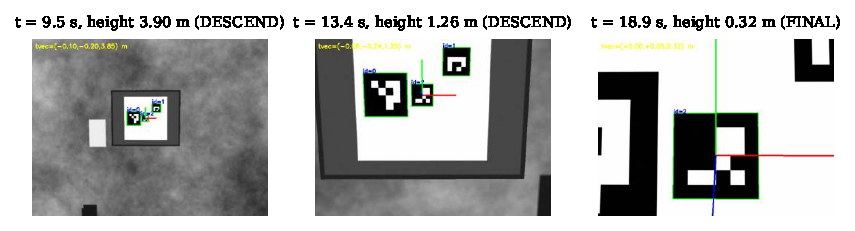
\includegraphics[width=\textwidth]{figures/camera_frames.pdf}
\caption{Rendered downward-camera frames from the ROS~2 run on the \emph{straight} scenario,
with detected markers outlined and the estimated pad axes drawn. Left: all three markers
visible at \SI{3.9}{m}. Middle: \SI{1.26}{m}. Right: \SI{0.32}{m}, where only the small
centre marker is fully in view.}
\label{fig:frames}
\end{figure*}

\subsection{Flight-controller state errors}
The estimator does not receive the true aircraft state. The reported attitude includes a slowly
varying bias (\ang{0.4} standard deviation, \SI{5}{s} correlation time) and white noise
(\ang{0.05}); the reported velocity has \SI{0.05}{m/s} white noise; and the reported position
drifts as a random walk of \SI{0.02}{m/\sqrt{s}}.

\subsection{Execution}
\label{sec:exec}
The same simulator, detector, estimators and controller are used in two ways: as the ROS~2
graph of Fig.~\ref{fig:arch}, run in Docker, and as a single-process batch runner with the same
camera rate and latency for Monte Carlo experiments. The simulation step is \SI{5}{ms}. An
interactive browser front end to the same code is also included; it exposes the parameters of
the vehicle, wind, aircraft, camera, pad, estimator and controller and was used for
exploration only, not for the results below.

%% ------------------------------------------------------------------------------------------
\section{Experiments}

\subsection{E1: pad speed from a hovering aircraft}
The aircraft holds position with the camera \SI{3.5}{m} above the deck while the vehicle drives
underneath in a straight line, \SI{0.6}{m} to one side, at a constant speed from 1 to
\SI{9}{m/s}, with three seeds per speed. Wind is active. All three estimators process the same
detections. The number of detections per pass falls from 103 at \SI{1}{m/s} to 13 at
\SI{9}{m/s}.

\begin{figure*}[t]
\centering
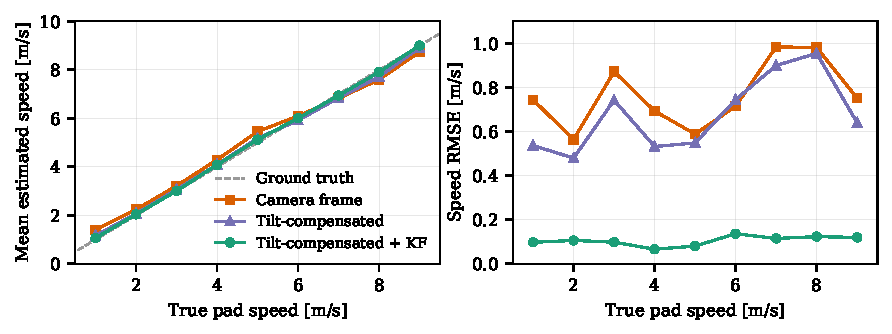
\includegraphics[width=\textwidth]{figures/speed_sweep.pdf}
\caption{E1. Left: mean estimated speed against true pad speed. Right: speed RMSE. Each point
averages three passes.}
\label{fig:speed}
\end{figure*}

Fig.~\ref{fig:speed} and Table~\ref{tab:speed} show the results. On average, AC and AC+KF
follow the true speed closely; CF overestimates at low speed (\SI{1.40}{m/s} for a
\SI{1}{m/s} pad) and is within \SI{0.5}{m/s} of the truth from \SI{2}{m/s} upward. The
finite-difference variants have an RMSE of
0.48--\SI{0.98}{m/s}, as each difference is taken over only \SI{33}{ms}. The Kalman filter
reduces the RMSE to 0.07--\SI{0.14}{m/s} at every speed. It produces no output for the first
fixes of each pass while it initialises (or re-initialises after a gap); this accounts for 3\% of samples at \SI{1}{m/s} and
up to 18\% at the higher speeds, where a pass contains fewer detections. The median error in
the direction of motion at \SI{1}{m/s} is \ang{31.2} for CF, \ang{10.1} for AC and \ang{1.8}
for AC+KF; at \SI{9}{m/s} the values are \ang{2.0}, \ang{0.9} and \ang{0.2}.

\begin{table}[t]
\centering
\caption{E1 speed estimation, hovering aircraft at \SI{3.5}{m}}
\label{tab:speed}
\footnotesize
\setlength{\tabcolsep}{2.5pt}
\begin{tabular}{@{}lccc@{}}
\toprule
Estimator & Mean at 1 / \SI{9}{m/s} & RMSE range & Median heading error \\
& [m/s] & [m/s] & at 1 / \SI{9}{m/s} \\
\midrule
CF & 1.40 / 8.74 & 0.56--0.98 & \ang{31.2} / \ang{2.0} \\
AC & 1.16 / 8.91 & 0.48--0.95 & \ang{10.1} / \ang{0.9} \\
AC+KF & 1.06 / 9.00 & 0.07--0.14 & \ang{1.8} / \ang{0.2} \\
\bottomrule
\end{tabular}
\end{table}

\subsection{E2: estimation accuracy in closed-loop flight}
The AC+KF variant flew the aircraft in all seven scenarios with four seeds each (28 runs, up
to \SI{60}{s} each), while the CF and AC variants ran in parallel on the same detections. This
gives 22\,092 detections (21\,681 with an AC+KF output), each compared with the true relative state at the image time.

\begin{table}[t]
\centering
\caption{E2 estimation error over 22\,092 in-flight detections}
\label{tab:est}
\begin{tabular}{@{}lcccc@{}}
\toprule
Estimator & \multicolumn{2}{c}{Position error [cm]} & Rel.\ speed & Altitude \\
& median & 95th pct. & MAE [m/s] & RMSE [cm] \\
\midrule
CF & 21.0 & 95.6 & 0.66 & 10.8 \\
AC & 1.4 & 5.5 & 0.15 & 2.5 \\
AC+KF & 2.2 & 6.4 & 0.07 & 1.9 \\
\bottomrule
\end{tabular}
\end{table}

\begin{figure*}[t]
\centering
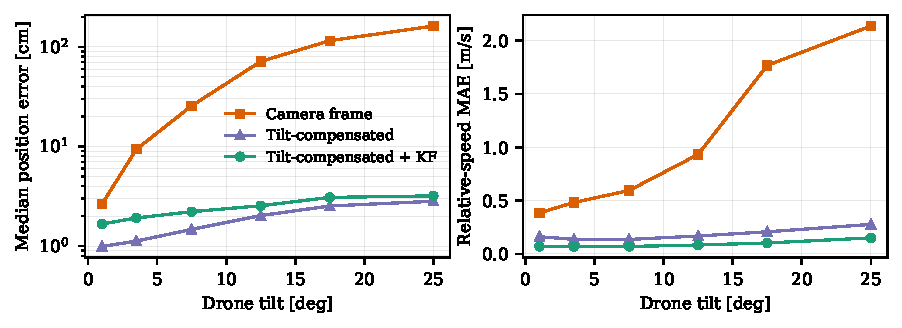
\includegraphics[width=\textwidth]{figures/error_vs_tilt.pdf}
\caption{E2. Median horizontal position error (left, log scale) and relative-speed mean
absolute error (right) against aircraft tilt at the image time, for detections in 28
closed-loop flights. Bins: \ang{0}--\ang{2}, \ang{2}--\ang{5}, \ang{5}--\ang{10},
\ang{10}--\ang{15}, \ang{15}--\ang{20}, \ang{20}--\ang{30} (1485, 6136, 10\,166, 3365, 681
and 259 detections for CF and AC; AC+KF has slightly fewer, as it gives no output while
initialising).}
\label{fig:tilt}
\end{figure*}

Table~\ref{tab:est} gives the overall errors and Fig.~\ref{fig:tilt} breaks them down by tilt.
The CF position error is \SI{2.6}{cm} below \ang{2} of tilt, \SI{25.6}{cm} at
\ang{5}--\ang{10}, \SI{71.5}{cm} at \ang{10}--\ang{15} and \SI{1.62}{m} at
\ang{20}--\ang{30}. This is the expected geometric effect: at height $h$, a tilt $\theta$
displaces the apparent pad position by about $h\tan\theta$. With attitude compensation the
median error stays between 1.0 and \SI{2.8}{cm} (AC) and between 1.7 and \SI{3.2}{cm}
(AC+KF) across all tilt bins. The filtered position is slightly less accurate than the raw
compensated position, because the filter smooths across frames, but its relative-speed error
is half as large (\SI{0.07}{} versus \SI{0.15}{m/s}), and its median error in the pad's ground
velocity is \SI{0.05}{m/s} against \SI{0.18}{m/s}. The CF altitude, taken directly as $t_z$,
has an RMSE of \SI{10.8}{cm}; after compensation it is \SI{1.9}{cm}.

\subsection{E3: closed-loop landing}
Each estimator variant in turn drives the controller in all seven scenarios with four seeds
(28 runs per variant, 84 in total). A run starts with the aircraft at \SI{6}{m} height,
\SI{2.5}{m} horizontally from the vehicle, and ends at touchdown, after \SI{60}{s}
(\emph{timeout}), or when the pad has not been seen for \SI{10}{s} after first being tracked
(\emph{lost}). A run counts as a landing only if the aircraft comes to rest on the pad, within
\SI{0.35}{m} of the centre, with a vertical impact speed of at most \SI{2.2}{m/s} and a
horizontal slip of at most \SI{0.6}{m/s} relative to the deck.

\begin{table}[t]
\centering
\caption{E3 closed-loop landings (successes out of 4 per scenario)}
\label{tab:land}
\setlength{\tabcolsep}{4pt}
\begin{tabular}{@{}lccccccc|c@{}}
\toprule
Estimator & stat. & str. & acc. & circ. & weave & s\&g & fast & total \\
\midrule
CF & 0 & 0 & 0 & 0 & 0 & 0 & 0 & 0/28 \\
AC & 2 & 1 & 2 & 1 & 0 & 0 & 0 & 6/28 \\
AC+KF & 3 & 2 & 1 & 1 & 0 & 0 & 0 & 7/28 \\
\bottomrule
\end{tabular}
\end{table}

Table~\ref{tab:land} summarises the outcomes. All 28 CF runs ended as \emph{lost}, with the pad
detected in 3.4\% of camera frames on average, against 74\% (AC) and 54\% (AC+KF). This is
consistent with the tilt-dependent CF error of Fig.~\ref{fig:tilt}: once the aircraft tilts
to follow the pad, the CF estimate places the pad tens of centimetres to metres from its true
position.

With attitude compensation, landings occurred on the static, straight, accelerating and circular motions. The seven AC+KF landings
ended a mean of \SI{6.3}{cm} (range 2.1--\SI{14.4}{cm}) from the pad centre, with vertical
impact speeds of 2.08--\SI{2.18}{m/s} and horizontal slip of 0.06--\SI{0.37}{m/s}. The six AC
landings ended a mean of \SI{5.3}{cm} (range 1.7--\SI{10.0}{cm}) from the centre. The mean
time to touchdown for AC+KF ranged from \SI{21.5}{s} (circle) to \SI{49.0}{s}
(accelerating).

The remaining AC+KF runs all ended in \emph{timeout} (21 of 28), as did 20 of the AC runs (the
other two AC failures were \emph{lost}). The failed AC+KF runs went through a mean of 1.95
abort-and-retry cycles. No variant landed in the \emph{weave}, \emph{stop\_go} or \emph{fast}
scenarios. The estimation errors of E2 include these failed runs, so the failures are not
explained by inaccurate estimates on frames in which the pad was detected. Every abort is
triggered from the DESCEND or FINAL state, that is, at low height, where the pad is detected
in fewer frames (Section~\ref{sec:vis}) and the controller relies more on the filter's
prediction. Identifying which abort condition dominates in each scenario is left to future
work.

\subsection{Full ROS~2 graph}
To check that the node graph behaves like the batch runner, single runs were flown through the
ROS~2 graph with AC+KF on four scenarios. The \emph{static} run landed after \SI{30.2}{s},
\SI{11.1}{cm} from the centre, at \SI{1.99}{m/s} vertical impact speed; the \emph{straight}
run landed after \SI{19.3}{s}, \SI{9.4}{cm} from the centre, at \SI{2.12}{m/s}. The
\emph{circle} and \emph{weave} runs timed out. Fig.~\ref{fig:run} shows the \emph{straight}
run.

\begin{figure}[t]
\centering
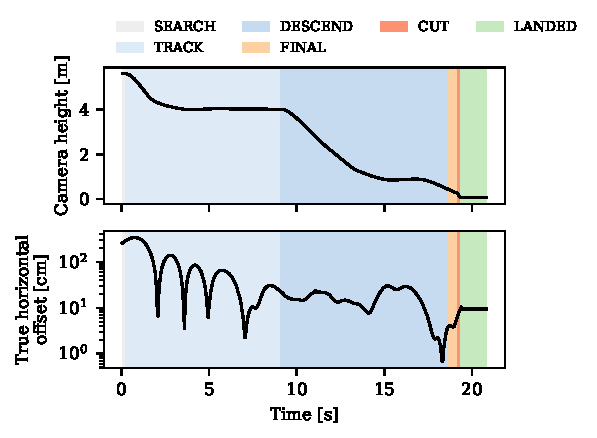
\includegraphics[width=\columnwidth]{figures/landing_run.pdf}
\caption{ROS~2 run on the \emph{straight} scenario (\SI{2}{m/s}) with AC+KF: camera height
and true horizontal offset between aircraft and pad, with the controller state shaded.}
\label{fig:run}
\end{figure}

\subsection{E4: pad visibility against height}
\label{sec:vis}
Fig.~\ref{fig:vis} shows, for all 28 AC+KF runs, the fraction of camera frames in which each
marker was detected, by camera height. Between \SI{1.2}{m} and \SI{4}{m} the pad was detected
in 86--90\% of frames, and all three markers contributed. Below \SI{0.8}{m} the large and
medium markers were detected in at most 23\% of frames, and most detections came from the
small centre marker. The overall detection rate fell to 67\% at 0.5--\SI{0.8}{m}, 39\% at
0.3--\SI{0.5}{m} and 11\% below \SI{0.3}{m}. Above \SI{5}{m} the pad was detected in only 1.5\% of frames; we did not
investigate the cause of this further.

\begin{figure}[t]
\centering
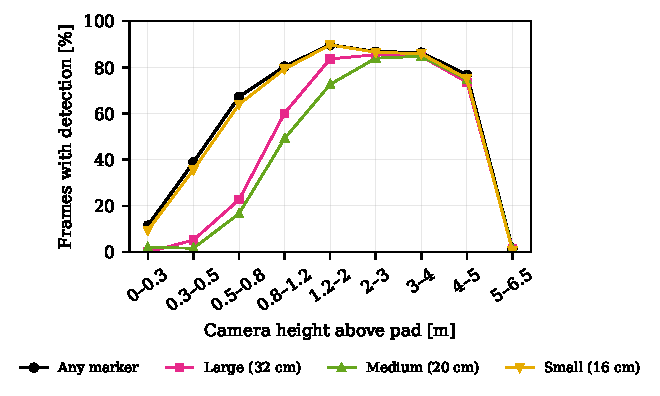
\includegraphics[width=\columnwidth]{figures/visibility.pdf}
\caption{E4. Fraction of camera frames with a detection of any pad marker and of each marker,
against camera height, over 28 closed-loop runs.}
\label{fig:vis}
\end{figure}

%% ------------------------------------------------------------------------------------------
\section{Discussion}

\emph{Attitude compensation.} The largest single effect in these experiments is the rotation
of the camera measurement by the aircraft attitude. Without it, the estimate is accurate only
while the aircraft is nearly level. That is the situation in a hover test such as E1, where
the CF variant's mean speed is within \SI{0.5}{m/s} of the truth from \SI{2}{m/s} upward, but not in closed-loop pursuit, where tilts of
\ang{5}--\ang{15} are routine (Fig.~\ref{fig:tilt}). In closed loop, none of the CF runs kept the pad in view. Compensation requires only the attitude that the flight controller
already estimates and a timestamp match between image and attitude.

\emph{Filtering.} The Kalman filter did not improve position accuracy, but it halved the
relative-speed error in flight and reduced the speed RMSE by a factor of 4.5 to 10.5 relative to the unfiltered variants in
the hover test.
This matters for the motor-cut decision, which extrapolates the relative velocity over the
fall time. The filter's prediction also supplies an estimate at the controller rate and
during short gaps in detection, which are frequent below \SI{0.5}{m}.

\emph{Pad design.} Using markers of several sizes kept the pad detectable over the whole
tracking range, as intended. The limiting factor is the final half metre, where the camera's
footprint becomes smaller than the pad. The \SI{16}{cm} centre marker is a compromise: a
smaller marker would remain in view at lower heights but is harder to detect from further
away, and a larger one leaves the frame sooner.

\emph{Landing success.} With accurate estimates, closed-loop landings succeeded for steady or
slowly changing vehicle motion, but the overall success rate was 25\% (7 of 28) for AC+KF and
no landings occurred for weaving, stop-and-go or fast motion. The mean vertical impact speed of
successful landings (about \SI{2.1}{m/s}) is close to the \SI{2.2}{m/s} limit, because the
motors are cut from a fixed hold height; the success count is likely to be sensitive to that limit
and to the cut height.

\emph{Limitations.} The results are from simulation only. The rendering uses flat textured
planes without lighting changes, lens distortion or motion blur from rotation. The aircraft
model is a velocity-controlled model rather than a rotor-level one, and ground effect and
deck motion (pitch and roll from the road) are not modelled. Each closed-loop configuration
was run with four seeds, so the per-scenario success counts in Table~\ref{tab:land} have
wide uncertainty; in particular, the difference between 6/28 and 7/28 for AC and AC+KF is not
meaningful at this sample size.

%% ------------------------------------------------------------------------------------------
\section{Conclusion}
We presented a vision-only system for landing a quadcopter on a moving ground vehicle, built
from a three-marker ArUco pad, attitude-compensated pose estimation, a constant-velocity
Kalman filter and a landing state machine with a predicted-impact check before the motor cut,
and evaluated it in a closed-loop simulator that runs the real marker detector on rendered
images. Attitude compensation reduced the median position error at \ang{20}--\ang{30} of tilt
from \SI{1.62}{m} to about \SI{3}{cm}, and no landing succeeded without it. In the hover
test, the Kalman filter brought the speed RMSE below \SI{0.15}{m/s} at all tested speeds. Landings
succeeded on stationary, straight, accelerating and circling vehicles, ending within
\SI{15}{cm} of the pad centre, but not on weaving, stop-and-go or fast vehicles.

Future work will address the final approach for manoeuvring vehicles, where the controller
currently aborts repeatedly, evaluate the pipeline on flight hardware, and replace the fixed
cut height with one chosen from the predicted impact speed.

\bibliographystyle{IEEEtran}
\bibliography{references}

\end{document}
